\chapter{RapidMiner}
\label{ch:anexo-b}
\newpage
%\blindtext[5]

RapidMiner es una herramienta de código abierto, usado para la minería de datos. Utiliza un ambiente gráfico que permite combinar distintos operadores y generar procesos de tratamiento y/o análisis de datos\\

Operadores utilizados en la creación del proceso para la predicción de la deserción.\\

\begin{longtable}{>{\centering\arraybackslash}m{3cm} >{\centering\arraybackslash}m{8cm}}
		\hline
		Operador & Descripción \\
		\hline \hline
		\endfirsthead
		
		\hline
		Operador & Descripción \\
		\hline \hline
		\endhead
		
		 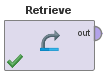
\includegraphics[width=20mm,height=20mm]{retrieve.png} & Este operador se utiliza para acceder a los repositorios. Transforma la mayor cantidad de datos del archivo de entrada en metadatos para un mejor procesamiento. \\	\hline \\
		
	     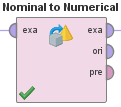
\includegraphics[width=20mm,height=20mm]{nominal.png} & Este operador cambia el tipo de atributos no numéricos seleccionados a un tipo numérico. También asigna todos los valores de estos atributos a valores numéricos. \\	\hline \\
		
	     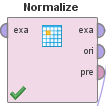
\includegraphics[width=20mm,height=20mm]{normalize.png} &  Este operador normaliza los valores de atributos de los atributos seleccionados.\\	\hline \\
		
	     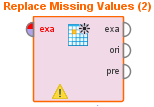
\includegraphics[width=20mm,height=20mm]{replace.png} & Este operador reemplaza los valores faltantes en los ejemplos de atributos seleccionados por un reemplazo especificado. \\ \hline \\
		
	     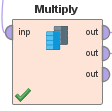
\includegraphics[width=20mm,height=20mm]{multiply.png} & Este operador copia su objeto de entrada a todos los puertos de salida conectados. No modifica el objeto de entrada. \\	\hline
		
	     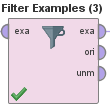
\includegraphics[width=20mm,height=20mm]{filter.png} & Este operador selecciona los datos de un conjunto de datos que se deben conservar y qué datos deben eliminarse. Se mantienen los datos que satisfacen la condición dada, se eliminan los datos restantes. \\	\hline \\
		
		 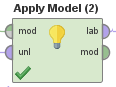
\includegraphics[width=20mm,height=20mm]{apply.png} & Este operador aplica un modelo ya aprendido o entrenado en un conjunto de datos. \\	\hline \\
		 
		 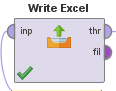
\includegraphics[width=20mm,height=20mm]{write.png} &  Este operador escribe el conjunto de datos en un archivo de hoja de cálculo de Excel.\\	\hline \\
		
		 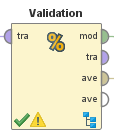
\includegraphics[width=20mm,height=20mm]{validation.png} & Este operador realiza una validación simple, es decir, divide aleatoriamente los datos en un conjunto de entrenamiento y un conjunto de pruebas y evalúa el modelo. Este operador realiza una validación de división para estimar el rendimiento de un operador de aprendizaje (normalmente en conjuntos de datos no vistos). Se utiliza principalmente para estimar la precisión con la que un modelo (aprendido por un operador de aprendizaje en particular) se llevará a cabo en la práctica. \\	\hline \\
		 
		 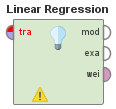
\includegraphics[width=20mm,height=20mm]{linear.png} & Este operador calcula un modelo de regresión lineal a partir de la entrada del conjunto de datos. \\	\hline \\
		 
		 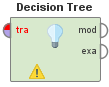
\includegraphics[width=20mm,height=20mm]{decision.png} & Genera un árbol de decisión para la clasificación de datos nominales y numéricos. \\	\hline \\
		 
		 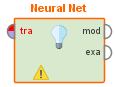
\includegraphics[width=20mm,height=20mm]{neural.png} & Este operador aprende un modelo por medio de una red neuronal feed-forward entrenada por un algoritmo de retropropagación (perceptron multicapa).  \\	\hline \\
		 
		 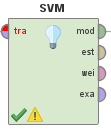
\includegraphics[width=20mm,height=20mm]{svm.png} & Este operador es un aprendiz de SVM (Support Vector Machine). Se basa en la implementación Java interna de mySVM por Stefan Rueping. \\	\hline \\
		 
		 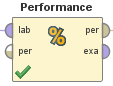
\includegraphics[width=20mm,height=20mm]{performance.png} & Este operador se utiliza para la evaluación del desempeño. Proporciona una lista de valores de criterios de rendimiento. Estos criterios de rendimiento se determinan automáticamente para adaptarse al tipo de tarea de aprendizaje. \\	\hline \\		

	\caption{Operadores RapidMiner}
	\label{tabla:operadores}
\end{longtable}